\documentclass{article}
\usepackage{iclr2026_conference,times}

\input{math_commands.tex}

\usepackage{hyperref}
\usepackage{url}
\usepackage{booktabs}
\usepackage{tabularx}
\usepackage{graphicx}
\usepackage{amsmath}
\usepackage{amssymb}
\usepackage{xspace}
\usepackage{enumitem}
\usepackage{xcolor}

\newcommand{\method}{\textsc{ExpertGym}\xspace}
\newcommand{\bcrc}{\textsc{BCRC}\xspace}
\newcommand{\rcfbc}{\textsc{RCF-BC}\xspace}
\newcommand{\tool}{\textsc{Tool}\xspace}
\newcommand{\memory}{\textsc{Memory}\xspace}
\newcommand{\code}{\textsc{Code}\xspace}
\newcommand{\rain}{\textsc{RAIN}\xspace}
\newcommand{\ram}{\textsc{RAM}\xspace}
\newcommand{\todo}[1]{\textcolor{gray}{[TODO: #1]}}

\title{ExpertGym: Behavior-Constrained Residual Composition for Agent Task Vectors}

% Anonymous submission.
\author{Anonymous Authors}

% \iclrfinalcopy
\begin{document}
\maketitle

\begin{abstract}
Task vectors are a promising interface for composing specialized language-model agents, but agent deltas are not task-pure capability packages: the same residual component may improve code execution while damaging tool-call formatting or memory-update behavior.  We propose \method, a mechanism-first framework for composing reinforced agent task vectors through \emph{behavior-constrained residual composition}.  Rather than learning a global expert coefficient or imitating expert traces, \method first diagnoses each residual entry by its span-conditioned utility and harm: successful versus failed code trajectories reveal capability directions, while tool-call spans and memory trajectories define protected behavior anchors.  A simple routing rule then adjusts residual coefficients only when capability evidence is present, shrinks positive deltas that harm protected behaviors, floors negative deltas that support protected behaviors, and leaves weak-evidence rows unchanged.  This view unifies insights from reasoning-preserving instruction merging and reinforced-agent preservation: task vectors provide capability priors, while behavior spans define where those priors may be safely expressed.  We present a reproducible evidence ledger over 588 residual entries and show that scalar coefficient shrinkage and hard role routing both miss important trade-offs, whereas a continuous residual field with behavior constraints exposes a more interpretable Pareto frontier across tool use, memory, and code.
\end{abstract}

\section{Introduction}

Specialized language-model agents are increasingly trained for executable behaviors: one model learns structured function calling, another learns multi-hop memory update, and another learns code generation under unit tests.  Deploying a router over all experts is expensive; full-parameter multitask reinforcement learning is slow and may erase expert-specific behaviors.  Model merging offers a lighter alternative: start from a base model $\theta_0$, compute expert task vectors $\Delta_e=\theta_e-\theta_0$, and form a single merged model.

For ordinary classification or instruction tuning, much of model merging can be treated as a geometric problem: align, trim, mask, average, or rescale task vectors to reduce parameter-space interference~\citep{ilharco2023editing,yadav2023ties,yu2023dare,deep2024della,gargiulo2025tsv,cheng2025wudi}.  Agent merging is harder.  A tool-use agent can have high next-token likelihood but output invalid JSON; a memory agent can answer a final question while corrupting intermediate state; a code agent can match an expert trajectory yet fail hidden tests.  The behavior of interest is not merely the average direction of a vector, but where the vector improves or damages executable spans.

This paper asks:

\begin{quote}
How should multiple agent task vectors be composed when their useful and harmful components are residual-level, span-conditioned, and behavior-dependent?
\end{quote}

Our answer is \method, a framework for \bcrc: behavior-constrained residual composition.  The central claim is intentionally simple:

\begin{quote}
Task vectors provide capability priors; behavior spans define where those priors may be safely expressed.
\end{quote}

\method differs from coefficient search.  It does not ask whether the \code expert should receive coefficient $0.5$ or $1.0$ globally.  Instead, it treats each residual entry $(p,e)$---a parameter group $p$ from expert $e$---as a unit of evidence.  Code pass/fail pairs tell us which residuals support executable code.  Tool-call spans and memory trajectories tell us which residuals should not be disrupted.  The resulting rule is deliberately minimal: increase capability-positive rows, shrink rows that harm protected behaviors, floor negative changes on behavior-supporting rows, and leave weak-evidence rows alone.

\paragraph{Positioning.}
\rain-Merging shows that instruction-tuned deltas can be injected into a reasoning model only after preserving the reasoning behavior subspace~\citep{huang2026rain}.  \ram studies behavior-knowledge preservation in reinforced agentic models~\citep{yuan2026ram}.  \method extends the same first principle to multi-agent composition: every executable skill defines both a capability direction and a behavior constraint.  The contribution is not a new optimizer, but a residual-level attribution protocol that explains why scalar gates, hard routing, and imitation-only objectives fail.

\paragraph{Contributions.}
\begin{itemize}[leftmargin=*]
    \item We identify a semantic mismatch between reasoning-preserving instruction merging and multi-expert agent merging: in \rain, the reasoning model is the protected anchor, whereas in \method the tool, memory, and code models are additive reinforced-agent deltas.
    \item We introduce \bcrc, a simple residual-level composition rule driven by capability utility and behavior harm on executable spans.
    \item We build an auditable residual evidence ledger over $588$ agent residual entries, connecting each coefficient decision to code pass/fail evidence, tool-call behavior, and memory trajectory preservation.
    \item We provide mechanism experiments showing that global code shrinkage and hard role routing can improve one metric while damaging another, motivating continuous residual fields under behavior constraints.
\end{itemize}

\section{Task-Vector Semantics}

The term ``task vector'' hides an important distinction.  Table~\ref{tab:semantic} summarizes the difference between \rain and the current \method setting.

\begin{table}[t]
\centering
\small
\begin{tabularx}{\linewidth}{lXX}
\toprule
Item & \rain-Merging & \method OP-VEC \\
\midrule
Anchor & DeepSeek-R1-Distill-Qwen-7B & Qwen2.5-7B-Instruct \\
Additive vector & Qwen2.5-Instruct $-$ Qwen2.5-Base & Tool / Memory / Code expert $-$ Qwen2.5-Instruct \\
Reasoning role & Protected target behavior, not an additive vector & Optional heterogeneous R1 delta \\
Control & Null-space projection + attention utility/harm alpha + lambda grid & Residual utility/harm routing over expert deltas \\
Main risk & Instruction delta leaks into reasoning format & Expert deltas conflict across executable behaviors \\
\bottomrule
\end{tabularx}
\caption{Task-vector semantics.  \rain adds projected instruction ability into a protected reasoning anchor.  \method composes multiple reinforced-agent capability priors relative to a shared instruction anchor.}
\label{tab:semantic}
\end{table}

This distinction matters empirically.  In the audited OP-VEC manifest, the three agent deltas have highly unequal norms:

\begin{equation}
    \|\Delta_{\code}\|_2=0.620,\quad
    \|\Delta_{\tool}\|_2=1.255,\quad
    \|\Delta_{\memory}\|_2=5.362.
\end{equation}

A raw R1/Math delta in the same OP-VEC slice has norm $347.068$, about $559.5\times$ the \code delta and $64.7\times$ the \memory delta.  Thus, a uniform coefficient is not a uniform capability injection, and a reasoning delta cannot be treated as a normal fourth expert without explicit scaling and behavior protection.

\section{Residual Capability Field}

Let $\mathcal{E}$ be a set of experts and $\mathcal{P}$ be residual entries such as layer-module groups.  A merged model is
\begin{equation}
    \theta(g)=\theta_0+\sum_{e\in\mathcal{E}}\sum_{p\in\mathcal{P}} g_{p,e}\Delta_{p,e}.
\end{equation}

The question is how to set $g_{p,e}$.  Scalar merging assumes $g_{p,e}$ is mostly a function of expert identity.  \method assumes it is a function of residual evidence:
\begin{equation}
    g_{p,e}=f(U_{p,e}, H_{p,e}, B_{p,e}),
\end{equation}
where $U$ is capability utility, $H$ is behavior harm, and $B$ is behavior support.

\paragraph{Residual response score.}
For a labeled behavior span $t$, let $h_{p,t}$ be the input activation to residual group $p$ and let
\begin{equation}
    u_{p,e,t}=\Delta W_{p,e}h_{p,t}
\end{equation}
be the response induced by expert $e$.  We record two quantities:
\begin{equation}
    E_{p,e,t}=\mathbb{E}\|u_{p,e,t}\|^2,\qquad
    S_{p,e,t}=\mathbb{E}[-\langle \nabla z_{p,t}, u_{p,e,t}\rangle],
\end{equation}
where $\nabla z_{p,t}$ is the gradient of the teacher-forced span loss with respect to the pre-residual hidden state.  $E$ asks whether the delta is expressed on the span; $S$ asks whether the expressed direction lowers the span loss to first order.  This is the concrete scoring primitive used in our evidence ledger.

\paragraph{Capability utility.}
For code, utility is measured by same-prompt successful and failed trajectories:
\begin{equation}
    U_{p,e}^{\code}=
    S_{p,e}(x,y^{+})-S_{p,e}(x,y^{-}),
\end{equation}
where $y^{+}$ passes the verifier and $y^{-}$ fails under the same prompt.  In practice we compute this contrast separately for prompt, reasoning, and final-code spans, then conservatively aggregate across sources so that a direction with strong source conflict is not treated as a clean code direction.

\paragraph{Behavior harm and support.}
Tool and memory define protected spans rather than ordinary scalar rewards.  A tool-call span should remain parseable and schema-correct; a memory trajectory should preserve update turns and final retrieval consistency.  We therefore score:
\begin{equation}
    H_{p,e}^{b}=\max(-S_{p,e,b},0),
    \qquad
    B_{p,e}^{b}=\max(S_{p,e,b},0),
\end{equation}
where $b$ is a protected behavior span such as tool call or memory trajectory.  Thus harm and support use the same first-order residual response as capability, but they play a different role: they constrain where a capability update is allowed to act.

\paragraph{Span-conditioned diagnostics.}
The current diagnostic workbench materializes this view as four auditable tables: $2016$ residual-response records, $2352$ gate records, $504$ pairwise interference records, and $73$ evaluation records.  Each row is keyed by an expert, layer, and module.  This is important because norm alone is misleading: a residual can be large but inactive on a behavior span, or active with the wrong sign.

The same analysis explains why code is difficult.  On the code-hurt subset, LiveBench prompt-span evidence and LiveCodeBench prompt-span evidence have Pearson correlation $-0.995$ across the $588$ residual entries, with a sign-conflict rate of $63.95\%$.  Thus, code is not a single smooth direction.  Prompt understanding, reasoning, and final-code spans can demand different residual signs, so a single code coefficient is structurally too coarse.

\begin{figure*}[t]
\centering
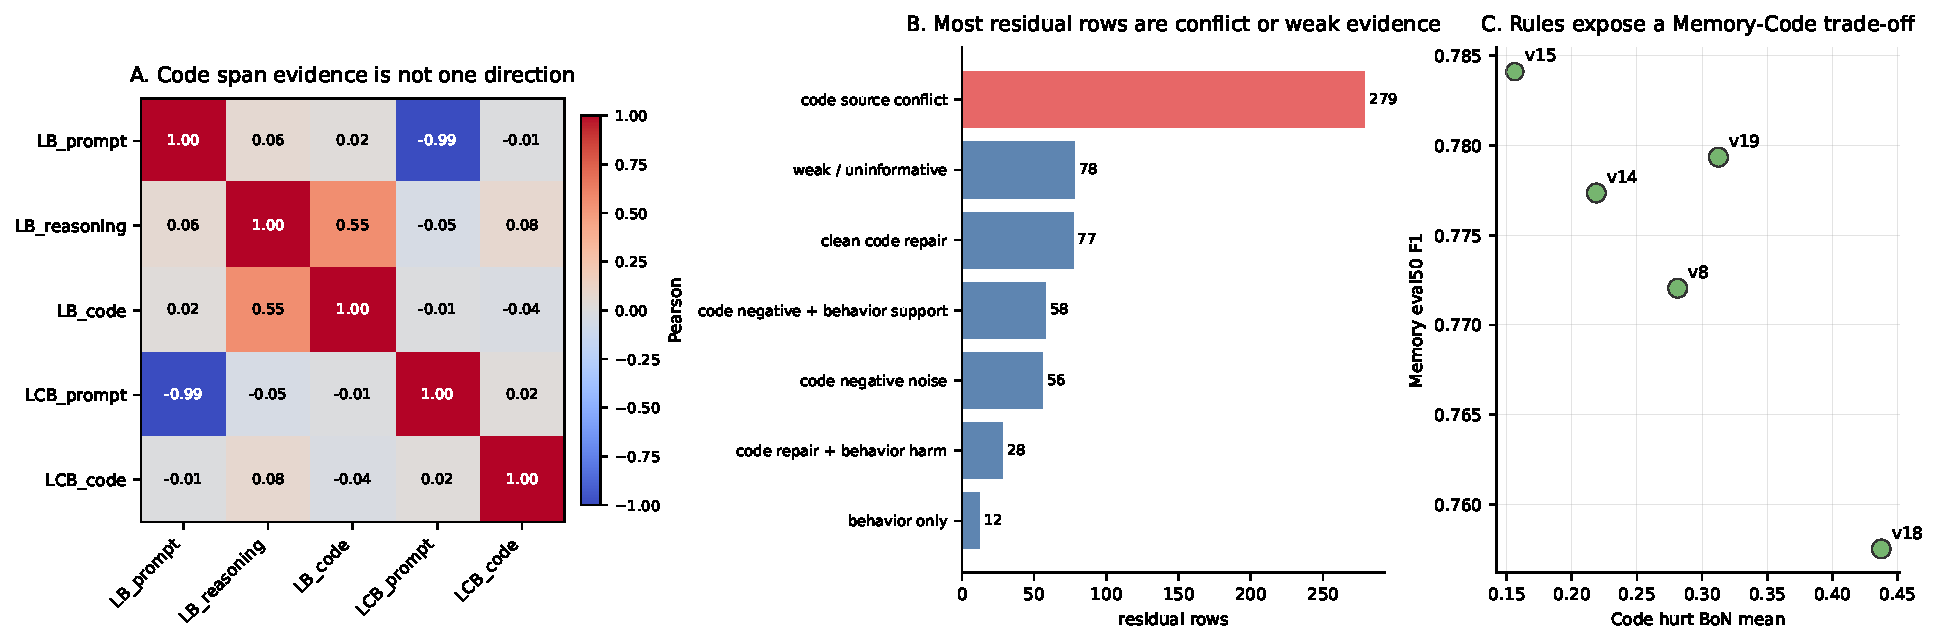
\includegraphics[width=\textwidth]{figures/diagnostic_residual_field.pdf}
\caption{\textbf{Residual diagnostics motivate behavior-constrained composition.}
Left: code evidence is source/span-conditioned; LiveBench prompt evidence and LiveCodeBench prompt evidence are nearly opposite directions.  Middle: most of the $588$ residual rows are conflict, weak-evidence, behavior-supporting, or noise-like rows rather than clean task rows.  Right: mechanism variants expose a Memory--Code trade-off; scalar code shrinkage improves memory but damages code, while soft behavior constraints keep a continuous code field.}
\label{fig:diagnostic-residual-field}
\end{figure*}

\paragraph{Pairwise-zero diagnosis.}
To avoid hiding mechanisms inside a three-expert aggregate, we also diagnose pairwise views: keep two experts and set the third expert's residual coefficients to zero.  These are diagnostic gates, not proposed methods.  They ask what kind of evidence would be removed by a scalar decision.  Figure~\ref{fig:pairwise-zero} shows that zeroing an expert does not remove a pure block.  Setting \code to zero removes $43$ code-repair rows and hurts code in existing ablations; setting \memory to zero removes $84$ memory-support rows; setting \tool to zero removes $126$ tool-support rows.  We mark missing behavior probes as N/A rather than zero conflict, since the current code contrast atlas does not contain direct \code-expert effects on tool or memory spans.  The diagnostic conclusion is therefore conservative: scalar zeroing is useful as a negative control, but the composition unit must remain residual-level and span-conditioned.

\begin{figure*}[t]
\centering
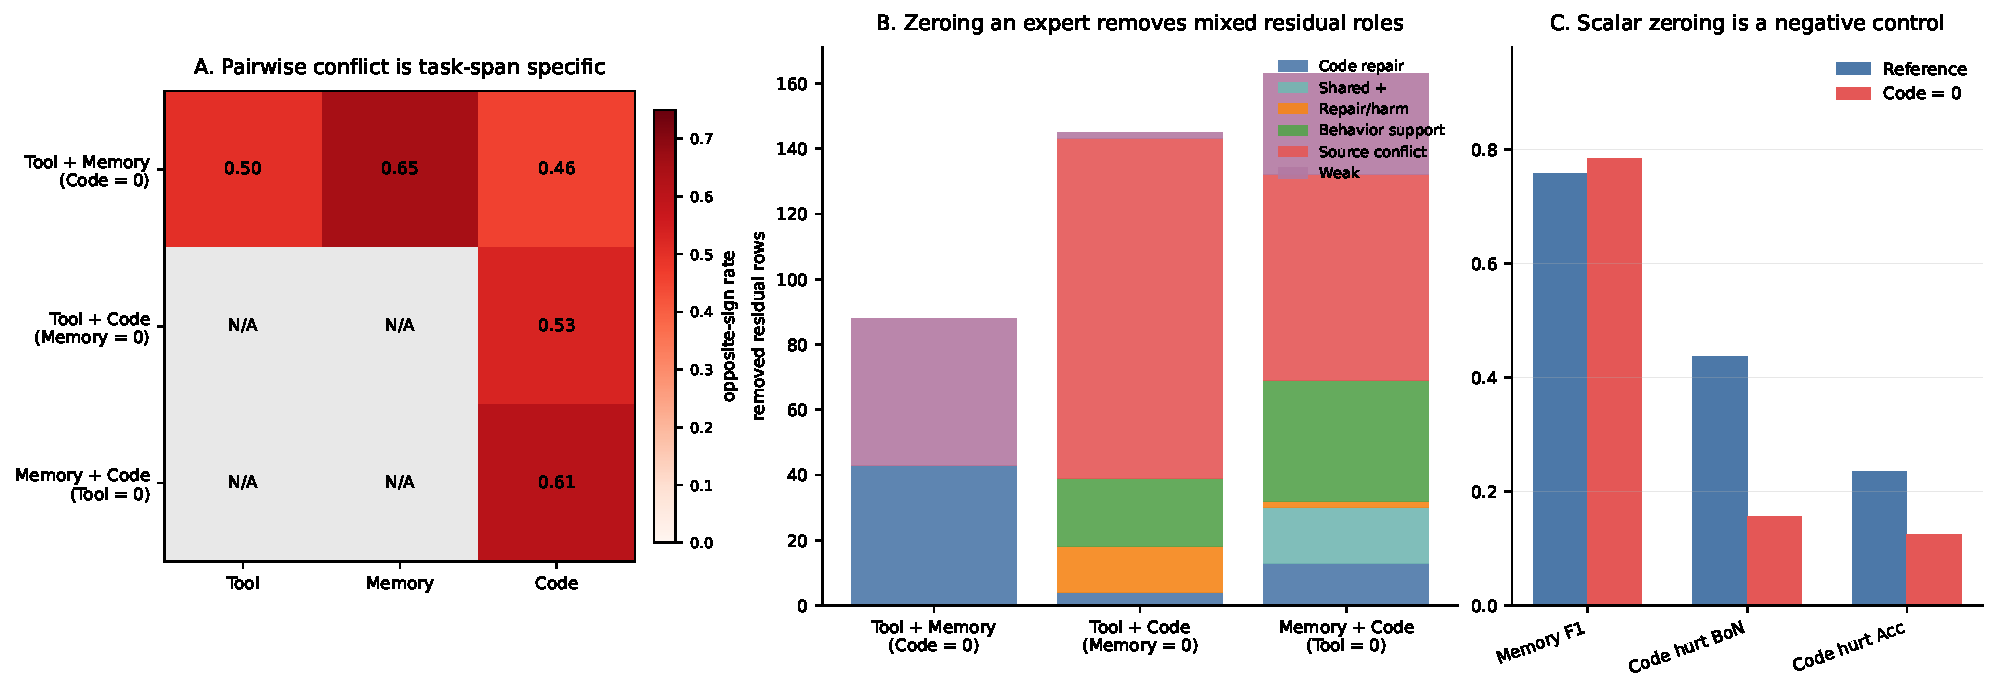
\includegraphics[width=\textwidth]{figures/pairwise_zero_diagnostics.pdf}
\caption{\textbf{Pairwise-zero diagnostics show why expert-level deletion is not a method.}
Left: pairwise opposite-sign rates are task-span specific; unavailable behavior probes are shown as N/A rather than as zero conflict.  Middle: zeroing one expert removes mixed residual roles, including code-repair, behavior-support, shared-positive, and source-conflict rows.  Right: the existing \code$=0$ ablation increases memory but damages code, making scalar zeroing a negative control rather than a composition rule.}
\label{fig:pairwise-zero}
\end{figure*}

\section{Behavior-Constrained Residual Composition}

\bcrc uses one rule for all agent skills.  Starting from a base gate $g^0$, for each residual row $(p,e)$:

\begin{enumerate}[leftmargin=*]
    \item If capability utility is positive, propose a positive delta.
    \item If the row harms a protected behavior, shrink the positive delta.
    \item If the row supports protected behavior, floor negative deltas at the base gate.
    \item If evidence is weak or contradictory, leave the row unchanged.
\end{enumerate}

In compact form, the implementation first forms a bounded capability update
\begin{equation}
    d_{p,e}=\mathrm{clip}(\alpha\,\widetilde{U}_{p,e},-\delta_{\max},\delta_{\max}),
\end{equation}
where $\widetilde{U}_{p,e}$ is a normalized signed utility score.  It is positive for residual rows supported by outcome contrast, negative for rows that consistently move failed trajectories closer than successful ones, and zero when evidence is weak or source-conflicted.  We then apply two behavior constraints:
\begin{equation}
d_{p,e}\leftarrow
\begin{cases}
\lambda_h d_{p,e}, & d_{p,e}>0 \ \mathrm{and}\ \max_b H^b_{p,e}>\tau_h,\\
0, & d_{p,e}<0 \ \mathrm{and}\ \max_b B^b_{p,e}>\tau_b,\\
d_{p,e}, & \mathrm{otherwise}.
\end{cases}
\end{equation}
The final coefficient is $g_{p,e}=\mathrm{clip}(g^0_{p,e}+d_{p,e},g_{\min},g_{\max})$.  Low-confidence or contradictory evidence sets $d_{p,e}=0$.  The current implementation instantiates this rule as \rcfbc:

\begin{itemize}[leftmargin=*]
    \item \textbf{Continuous code field}: pass/fail contrast supplies positive and negative code deltas.
    \item \textbf{Behavior utility floor}: tool/memory-supporting rows cannot receive harmful negative code updates.
    \item \textbf{Behavior harm veto}: rows that harm tool or memory have positive code deltas softened rather than blindly amplified.
\end{itemize}

\paragraph{Algorithmic form.}
The procedure is deliberately small and auditable:

\begin{center}
\fbox{
\begin{minipage}{0.94\linewidth}
\textbf{Behavior-Constrained Residual Composition.}
\begin{enumerate}[leftmargin=*]
    \item \textbf{Inputs}: base model $\theta_0$, expert deltas $\{\Delta_e\}$, residual groups $\mathcal{P}$, base gate $g^0$, and a small set of behavior probes with span labels.
    \item \textbf{Residual response}: for each $(p,e)$ and labeled span $t$, record $u_{p,e,t}=\Delta W_{p,e}h_{p,t}$.
    \item \textbf{Capability evidence}: estimate $U_{p,e}$ from same-prompt outcome contrast, e.g., pass trajectories minus fail trajectories for code.
    \item \textbf{Behavior evidence}: estimate $B_{p,e}$ and $H_{p,e}$ from the same signed-effect score on protected spans such as tool calls and memory trajectories.
    \item \textbf{Conservative update}: propose a bounded update from $U_{p,e}$; shrink positive updates when $H_{p,e}$ is high; floor negative updates when $B_{p,e}$ is high; leave low-confidence or contradictory rows at $g^0$.
    \item \textbf{Output}: a merged checkpoint $\theta(g)=\theta_0+\sum_{e,p}g_{p,e}\Delta_{p,e}$ and an evidence ledger explaining every changed residual row.
\end{enumerate}
\end{minipage}
}
\end{center}

This algorithm makes the calibration set a diagnostic instrument rather than a small training set.  A probe is useful only if it reveals whether a residual row supports or harms a behavior span; it is not used to memorize answers or to sweep a validation metric.

\section{Experimental Protocol}

The experiment design follows the mechanism-first claim.

\paragraph{D1: vector semantics audit.}
We first determine whether task vectors are commensurate.  This includes anchor model, additive vector definition, selected modules, norm distribution, and whether the behavior model is additive or protected.

\paragraph{D2: residual evidence atlas.}
For each residual row, we compute or record capability utility, behavior harm, behavior support, and the resulting routing decision.  The output is an auditable ledger rather than an opaque learned checkpoint.

The atlas assigns each residual entry to mechanism-facing roles such as clean code repair, shared positive residual, code repair with protected-behavior harm, code-negative but behavior-supporting residual, source-conflicted code residual, and uninformative residual.  These roles are not used as hard labels in the main method; they are diagnostics that tell us which simple routing rules are defensible.

\paragraph{D3: counterfactual residual intervention.}
We test whether changing predicted row groups moves metrics in the predicted direction.  Valid interventions are restricted to shrink predicted-harm rows, restore predicted-behavior rows, or amplify predicted-clean-capability rows.  This avoids post-hoc metric-targeted sweep.

\paragraph{Heldout discipline.}
We separate probes, monitors, guards, and formal evaluation.  Probe prompts may influence residual evidence and gate decisions, but cannot be reported as final metrics.  Monitor prompts may select among pre-declared variants, but receive no gradient and do not change the method.  Guard prompts are non-regression checks.  Formal Tool/Memory/Code evaluation is used only after the candidate set is frozen.  Diagnostic eval-leak experiments are allowed for failure analysis, but are excluded from paper-main tables.

\paragraph{Main evaluation.}
We evaluate tool use, memory, and code:

\begin{itemize}[leftmargin=*]
    \item \tool: BFCL-style function calling and ToolRL-80 stability.
    \item \memory: HotpotQA / MemAgent-compatible memory F1.
    \item \code: CURE / LiveBench / LiveCodeBench diagnostic subsets, reporting pass@1 and BoN separately.
\end{itemize}

\section{Experiments}

The experiments are organized around three questions rather than a single leaderboard number.  \textbf{Q1}: do agent task vectors contain residual-level, span-conditioned utility and harm?  \textbf{Q2}: does this diagnosis explain why expert-level scaling and zeroing are too coarse?  \textbf{Q3}: does the resulting behavior-constrained field give an auditable operating point under the same Tool/Memory/Code evaluation harness?

\paragraph{Diagnostic setup.}
Table~\ref{tab:main-evidence} summarizes the mechanism candidates used to answer Q1 and Q2.  These rows use quick Tool/Memory metrics and a code-hurt subset; they are not a final benchmark table.  Their role is to test whether predicted residual groups move metrics in the predicted direction.

Two diagnostic facts guide the interpretation.  First, only $60/588$ residual entries are clean code-repair rows, while $167/588$ are code-source-conflict rows that also carry tool or memory behavior evidence.  Second, the code-memory expert pair has the largest observed conflict in the diagnostic workbench.  These facts rule out the simplest scalar story: the issue is not whether to ``add code'' or ``add memory'', but where a residual helps one executable behavior while hurting another.

The pairwise-zero diagnostic in Figure~\ref{fig:pairwise-zero} gives the same conclusion from a different angle.  Removing an expert always deletes a mixture of rows.  The \code-zero ablation removes clean code-repair evidence; the \memory-zero view removes memory-support rows; the \tool-zero view removes tool-call behavior anchors.  Thus, zeroing or shrinking a whole expert can expose a trade-off, but it is too coarse to define the final composition rule.

\begin{table*}[t]
\centering
\scriptsize
\resizebox{\textwidth}{!}{%
\begin{tabular}{llccccc}
\toprule
Candidate & Rule & Changed & Tool mean & Memory F1 & LB acc/BoN & LCB acc/BoN \\
\midrule
v8 & Code field + hard Tool/Memory veto & 135 & 0.7944 & 0.7720 & 0.0938 / 0.2500 & 0.2969 / 0.3125 \\
v18 & Continuous field + soft behavior constraints & 205 & 0.7931 & 0.7575 & 0.1406 / 0.2500 & 0.3281 / 0.6250 \\
v19 & Strict archetype cleanup & 173 & 0.7956 & 0.7793 & 0.1250 / 0.1875 & 0.3281 / 0.4375 \\
v14 & Global code coefficients $\times 0.5$ & 320 & 0.7944 & 0.7774 & 0.2031 / 0.2500 & 0.2500 / 0.1875 \\
v15 & Global code coefficients $=0$ & 320 & 0.7800 & 0.7841 & 0.0781 / 0.1250 & 0.1719 / 0.1875 \\
v20 & Local weak/noise code rows $\times 0.5$ & 60 & 0.7944 & 0.7772 & 0.0781 / 0.1250 & 0.3125 / 0.5000 \\
v21 & Local weak/noise code rows $=0$ & 60 & 0.7931 & 0.7664 & 0.1250 / 0.3750 & 0.2500 / 0.2500 \\
\bottomrule
\end{tabular}
}
\caption{Mechanism evidence.  Hard behavior constraints protect memory but suppress code; global code shrinkage improves memory but damages code; local hard masking is more targeted but still loses source-specific code signal.  \rcfbc keeps a continuous field and exposes the trade-off instead of collapsing it into one expert scalar.}
\label{tab:main-evidence}
\end{table*}

The strongest negative control is global code shrinkage.  Setting the code expert to zero improves memory F1 from $0.7575$ to $0.7841$, but LiveCodeBench BoN drops from $0.6250$ to $0.1875$.  This supports the central claim: code residuals cannot be treated as a disposable scalar block.  Conversely, strict archetype cleanup improves memory but loses part of the code field, showing that hard semantic labels are insufficient.  The useful object is a continuous residual field under behavior constraints.

Counterfactual interventions provide the next layer of evidence.  Halving only $60$ low-confidence code rows recovers nearly the same memory gain as global code-half, but still damages parts of code; hard-masking those rows gives a smaller memory gain and reduces LiveCodeBench relative to the soft field.  Splitting this into negative-noise rows and weak rows produces non-additive effects, indicating that residual groups interact and cannot be pruned independently by a single hard label.  Therefore, ``harmful'' in one diagnostic source is not enough to justify deletion: a row should be hard-masked only when negative evidence is source-consistent, expressed on the target span, and unsupported by protected behaviors.  This is why \bcrc uses behavior-constrained soft updates rather than a pure harmful-residual mask.

\paragraph{Full Eval6 sanity check.}
For Q3, we freeze a minimum candidate set and run the same Eval6-style Tool/Memory/Code harness for the soft behavior-constrained field and two principled ablations.  Table~\ref{tab:eval6-family} gives the completed queue.  The result narrows the claim: the soft behavior-constrained field has the highest Code pass@1 and worst-task score inside this BCRC-family queue, but the no-behavior ablation has the highest simple average.  Thus, the current evidence supports an interpretable trade-off-control claim rather than a broad SOTA claim.

\begin{table*}[t]
\centering
\scriptsize
\resizebox{\textwidth}{!}{%
\begin{tabular}{llccccccc}
\toprule
Candidate & Role & Tool & Tool live & Memory F1 & Code Acc & Code BoN & Avg & Worst \\
\midrule
BCRC v18/v9 & Soft behavior-constrained residual field & 0.7931 & 0.7188 & 0.7570 & 0.3301 & 0.3939 & 0.6267 & 0.3301 \\
No behavior & Code field without behavior constraint & 0.7956 & 0.7188 & 0.7650 & 0.3260 & 0.4076 & 0.6289 & 0.3260 \\
Hard behavior & Hard Tool/Memory behavior constraint & 0.7919 & 0.7188 & 0.7568 & 0.3274 & 0.4047 & 0.6254 & 0.3274 \\
\bottomrule
\end{tabular}
}
\caption{Completed selected Eval6 queue.  Soft behavior constraints improve Code pass@1 and the worst-task score within the selected BCRC-family rows, while the no-behavior ablation has the highest simple average.  This supports a mechanism and trade-off-control claim, not a broad SOTA claim.}
\label{tab:eval6-family}
\end{table*}

\section{Discussion}

\paragraph{Why not only learn gates with RL?}
Earlier coefficient-learning experiments showed that executable rewards are sparse and saturated: many prompts are all-success, all-fail, or recoverable only through an expert trajectory.  This makes pure on-policy gate learning slow and unstable.  \bcrc uses rollouts and verifiers as diagnostic probes rather than as a high-variance end-to-end optimizer.

\paragraph{Why not use hidden-state imitation?}
Imitation can make the merged model closer to an expert without knowing whether that expert behavior is needed or whether it harms another task.  \method uses same-prompt pass/fail and protected behavior spans, so expert traces are evidence, not universal targets.

\paragraph{Relation to \rain and \ram.}
\rain can be read as one special case: instruction ability is injected only after preserving reasoning behavior.  \ram motivates preserving behavior knowledge in reinforced agents.  \method generalizes this principle across multiple agent skills: every expert delta is a capability prior, and every executable behavior can define a protected subspace.

\section{Limitations and Next Steps}

The current evidence is strongest as a mechanism study, not as a broad benchmark SOTA result.  Code remains difficult because pass@1 and BoN can move differently, and live code evaluation is expensive.  The next version should complete two items before submission:

\begin{enumerate}[leftmargin=*]
    \item Add RAM artifacts to the vector-semantics audit.
    \item Decide whether ToolRL-80 should be part of the main benchmark table or kept as an auxiliary tool-format stability check.
\end{enumerate}

\section{Conclusion}

\method reframes agent task-vector merging as residual-level capability attribution under behavior constraints.  The key insight is simple: task vectors are useful priors, but agent behaviors define where those priors are allowed to act.  This first-principles view explains why scalar coefficients and hard routing are brittle, and it provides a path toward interpretable, verifier-grounded composition of tool, memory, and code agents.

\bibliography{references}
\bibliographystyle{iclr2026_conference}

\end{document}
